\documentclass[10pt,a4paper]{article}


\usepackage[T1]{fontenc}
\usepackage[utf8]{inputenc}
\usepackage[english]{babel}
\usepackage[english]{isodate}
\usepackage[parfill]{parskip}
\usepackage[margin=3.cm]{geometry}
\usepackage{graphicx}
\graphicspath{{./figs/}}
\usepackage{amsmath}
\usepackage{amssymb}
\usepackage{cite}

\usepackage{xcolor}
\usepackage[caption=false]{subfig}
\usepackage{caption}
%\usepackage{orcidlink}
\usepackage{hyperref}
\hypersetup{
	colorlinks = true,
	urlcolor   = blue,
	citecolor  = black,
	linkcolor = black
}

\title{MyPTV user manual}



\begin{document}
	
\maketitle

\pagenumbering{Roman}
\tableofcontents
\newpage

\pagenumbering{arabic}







\section{3D-PTV principles}


The 3D-PTV method is used to measure trajectories of particles in 3D space. It utilises the pronciples of stereoscopic vision in order to reconstruc 3D positions of particles from images taken from several angles. A scheme of a typical 3D-PTV experiment using a four camera system is shown in Fig.~\ref{fig:3dptv_exp}. The "work horse" behind the 3D-PTV method is the colinearity condition, the 3D model. In principle, if we know what is the position and what is the orientation of the camera in 3D space ($O'$ and $\theta$ in Fig.~\ref{fig:3dmodel}), we can use the pin-hole camera model to relate the image space coordinates of a particle ($\eta,\, \zeta$ in Fig.~\ref{fig:3dmodel}) to the ray of light connecting the imaging center and the particle. Then, if we have more than one camera, the particle will be located at the intersection of the two rays. Detailed information is given in \cite{Virant1997, Mass1993}.  


\begin{figure}[h!]
	\centering
	\subfloat[]{\label{fig:3dptv_exp}
		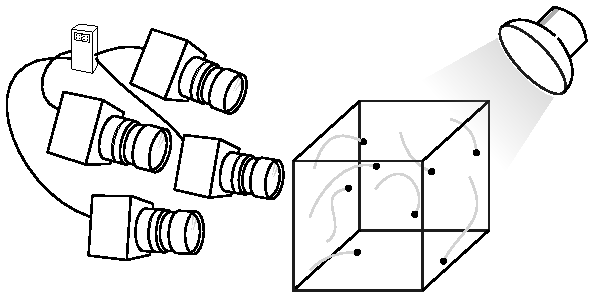
\includegraphics[width=6.5cm]{3D_PTV_acquisition.pdf}}
	\hfill
	%
	\subfloat[]{\label{fig:3dmodel}
		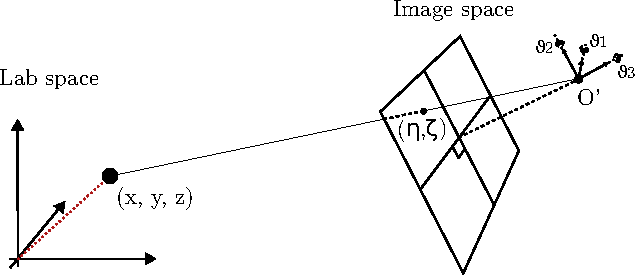
\includegraphics[width=6.5cm]{pinhole_model.pdf}}
	%
	\caption{(a) A schematics of a 3D-PTV experiment. (b) A schematic description of the 3d model, the pin-hole camera model.}
\end{figure}



Once the experiment, namely data aquisition, is done, there are six intrinsic steps to follow in order to complete the analysis. The six steps are outlined in Fig.~\ref{fig:steps}. In Camera calibration, we use images of known calibration targets to estimate the position, orientation and internal parameters of the cameras. In particle segmentation we use image analysis to obtain the paritlces' image space coordinates ($\eta, \, \zeta$). In the Particle matching step we use the ray crossing principle to decide which particle image in each of the cameras correspond to the same physical particle, and triagulate their positions through stereo mathcing. In particle tracking we connect the positions of particles in 3D space to form trajectories. In data conditioning we might use smoothing and re-tracking algorithms to enhance the quality of our data according to some physical heuristics. Lastly, we can analyze the data to obtain information on the physics of the particles we are studying. The MyPTV package is meant to handle the first five of these steps.    



\begin{figure}
	\centering
	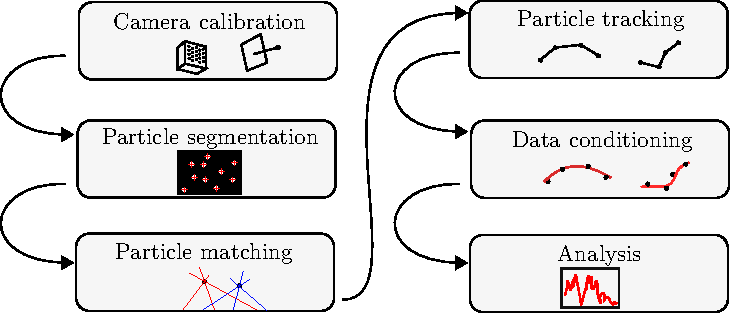
\includegraphics[width=10cm]{steps.pdf}
	\caption{Basic steps in the analysis of PTV raw data into particl trajectories and scientific output. The first five steps are handled by MyPYV. \label{fig:steps}}
\end{figure}


The sections that follow outline the code used to handle the 3D-PTV method in MyPTV.







\section{Imaging module - \texttt{imaging\char`_mod.py}}


The imaging module is used to handle the translation from 2D image space coordinates to lab spcae coordinates and vice-versa. For that, we use the following mathematical model:
%
\begin{equation}
\vec{r}-\vec{O} = \Big( \, 
\begin{bmatrix}
\eta + x_h\\
\zeta + y_h \\
f
\end{bmatrix}
+ \vec{e}(\eta, \zeta) \,\Big) \cdot \Big[ R \Big]
\label{eq:3dmodel}
\end{equation}
%
where the description of the notations is given in Table~\ref{tab1:mathdesc}. The matrix $[R]= [R_1]\cdot [R_2] \cdot [R_3]$ is the rotation matrix calculated with the components of the orientation vector, $\vec{\theta} = [\theta 1,\, \theta 2,\, \theta 3]$. In addition, the correction temr $\vec{e}$ is assumed to be a quadratic polynomial of the image space coordinates:
%
\begin{equation}
\vec{e}(\eta,\,\zeta) = [E]\cdot P(\eta,\,\zeta) =
\begin{bmatrix}
E_{11} & E_{12} & E_{13} & E_{14} & E_{15}\\
E_{21} & E_{22} & E_{23} & E_{24} & E_{25}\\
0 & 0 & 0 & 0 & 0
\end{bmatrix}
\cdot 
\begin{bmatrix}
\eta\\
\zeta\\
\eta^2\\
\zeta^2\\
\eta\,\zeta
\end{bmatrix}
\end{equation}
%
where $[E]$ is a $3\times5$ matrix that holds the correction coefficients; the last row is filled with zeros because we do not attempt to correct $f$.





\begin{table}
	\centering
	\caption{Description of mathematical notation. \label{tab1:mathdesc}}
	\begin{tabular}{p{5em} p{30em}}
		 \hline
		Symbol & Description \\ \hline
		$\vec{r}$ & Particle position in the lab space coorindates\\
		$\vec{O} $& Position of a camera's imaging center \\
		$\eta, \, \zeta$ & image space coordinates (pixels) of a particle \\
		$x_h , \, y_h$ & Correction to the camera's imaging center (in pixels)\\
		$f$ & The camera's principle distance divided by the pixel size \\ 
		$\vec{e}(\eta, \zeta)$ & A nonlinear correction term to compensate for image distortion and multimedia problems.\\
		$[R]$ & The roation matrix which corresponds to the camera orientation vector. \\  \hline
	\end{tabular}
\end{table}






\subsection{The \texttt{camera} object}

An object that stores the camera external and internal parameters and handles the projections to and from image space and lab space. Inputs are:

\begin{enumerate}
	\item \texttt{name} - string, name for the camera. This is the name used when saveing and loading the camera parameters.
	\item \texttt{resolution} - tuple (2), two integers for the camera number of pixels
	\item \texttt{cal\char`_points\char`_fname} - string (optional), path to a file with calibration coordinates for the camera.
\end{enumerate}


The important functionalities are:


\begin{enumerate}
	\item \texttt{get\char`_r(eta, zeta)} - Will solve eq.~\ref{eq:3dmodel} for the orientation vector $\vec{b} = \vec{r} - \vec{O}$, given an input of pixel coordinates $(\eta, \, \zeta)$.
	
	\item \texttt{projection(x)} - Will reverse solve equation~\eqref{eq:3dmodel} to find the image space coordinates $(\eta, \, \zeta)$, of an input 3D point, (\texttt{x=}$\vec{r}$).
	
	\item \texttt{save(dir\char`_path)} - Will save the camera parameters in a file called after the camera name in the given directory path, see Fig.~\ref{fig:camfiles}.
	
	\item \texttt{load(dir\char`_path)} - Will load the camera parameters in a file called after the camera name in the given directory path, see Fig.~\ref{fig:camfiles}.
\end{enumerate}



After calibration we can save the camera parameters on the hard disc. The camera files have the structure shown in Fig.~\ref{fig:camfiles}.

\begin{figure}
	\centering
	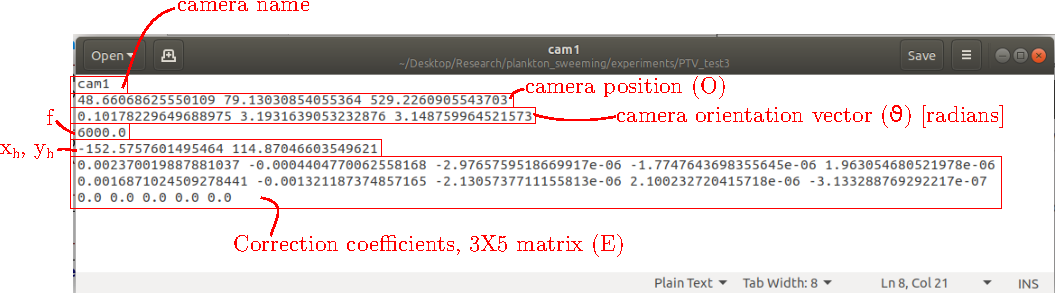
\includegraphics[width=\textwidth]{camera_files.pdf}
	\caption{The structure of a camera file. The files are simple text files where each row corresponds to a specific paramter and the values in each row are separated by a whitespace. \label{fig:camfiles}}
\end{figure}








\subsection{The \texttt{imsys} object}


An object that holds several camera instances and can be used to perform stereo-matching. The important functionalities are:


\begin{enumerate}
	\item \texttt{stereo\char`_match(coords, d\char`_max)} - Takes as an input a dicionary with coordinates in image space from the several cameras and calculates the triagulation position. \\ The coordinate dicitonary has keys that are the camera number and the values which are the coordinates in each camera. d\char`_max is maximum allowable distance for the triangulation.
	
\end{enumerate}








\section{Camera calibration - \texttt{calibrate\char`_mod.py}}


Holds the \texttt{calibrate} object that is used to find the camera calibration parameters.



\subsection{The \texttt{calibrate} object}

Used to solve for the camera parameters given an input list of image space and lab space coordinates. The inputs are:

\begin{enumerate}
	\item \texttt{camera} - An instance of a \texttt{camera} object which we would like to calibrate.
	\item \texttt{lab\char`_coords} - a list of lab space coordinates of some known calibration target. 
	\item \texttt{img\char`_coords} - a list of image space coordinates that is ordered in accordance with the lab space coordinates. 
\end{enumerate}



The important functionalities are:
%
\begin{enumerate}
	
	\item \texttt{searchCalibration(maxiter=5000, fix\char`_f=True)} - When this is run, we use a nonlinear least squares search to find the camera parameters that minimize the cost function (item 3 below). This function is used to find the $\vec{O}$, $\vec{\theta}$, $f$, and $x_h, \, y_h$ parameters (in case \texttt{fix\char`_f=False}, it will not solve for $f$. \texttt{maxiter} is the maximum number of iterations allowed for the least squares search.
	
	\item \texttt{fineCalibration(maxiter=500)} - This function will solve for the coefficients of the quadratic polynomial used for the nonlinear correction term ($[E]$). 
	
	\item \texttt{mean\char`_squared\char`_err} - This is our cost function, being the sum of distances between the image space coordinates and the projection of the given lab space coordinates.
	
\end{enumerate}
%
To find an optomal calibration solution, we might need to run each function several times, and run the coarse and fine calibrations one after the other until a satisfactory solution is obtained. Once it is obtained, we should keep in mind to save the results using the \texttt{save} functionality of the \texttt{camera} object. 







\bibliography{bib_myPTV}
\bibliographystyle{unsrt}

\end{document}